\documentclass{beamer}

% this is for coloring code correctly
\usepackage{listings}
\usepackage{courier}

% for multiline comment
\usepackage{verbatim} 

\usepackage{multirow}

% bold math
\usepackage{bm}

%http://tex.stackexchange.com/questions/29664/latex-error-unknown-graphics-extension-eps
\usepackage{epstopdf}

% add new font size
\makeatletter
\ifcase \@ptsize \relax% 10pt
  \newcommand{\miniscule}{\@setfontsize\miniscule{3}{4}}% \tiny: 5/6
\or% 11pt
  \newcommand{\miniscule}{\@setfontsize\miniscule{4}{5}}% \tiny: 6/7
\or% 12pt
  \newcommand{\miniscule}{\@setfontsize\miniscule{4}{5}}% \tiny: 6/7
\fi
\makeatother

% add new font size
\makeatletter
\ifcase \@ptsize \relax% 10pt
  \newcommand{\mini}{\@setfontsize\mini{4}{5}}% \tiny: 5/6
\or% 11pt
  \newcommand{\mini}{\@setfontsize\mini{5}{6}}% \tiny: 6/7
\or% 12pt
  \newcommand{\mini}{\@setfontsize\mini{5}{6}}% \tiny: 6/7
\fi
\makeatother

% http://tex.stackexchange.com/questions/33685/set-the-font-family-for-lstlisting
\lstset{
  basicstyle=\tiny\ttfamily,
  breaklines=true,
  numbers=left,
  stepnumber=1,
  numberstyle=\miniscule\color{gray}
}

% Aaron Robinson: my custimizations
% add padding to frametitle so that it's in the appropriate area of the background
\addtobeamertemplate{frametitle}{\vskip1ex\hspace*{1.8em}}{}
% remove navigation: http://stackoverflow.com/questions/3210205/how-to-get-rid-of-navigation-bars-in-beamer
\beamertemplatenavigationsymbolsempty
% force frametitle color to be white to go with background
\setbeamercolor{frametitle}{fg=white}

%http://tex.stackexchange.com/questions/7916/how-to-insert-a-background-image-in-a-beamer-frame
%Global Background must be put in preamble
\usebackgroundtemplate{
\includegraphics[width=\paperwidth,height=\paperheight]{pnnl_background.pdf}}

\institute{
Chemical \& Biological Signature Science \\
\vspace{3pt} National Security Directorate %\\
%Pacific Northwest National Laboratory
}

\author{Aaron Robinson} 
\title{\LARGE Python \& SQLite}

\begin{document}
%%%%%%%%%%%%%%%%%%%%%%%%%%%%%%%%%%%
\begin{frame}[plain] % 'plain' suppresses header & footer decorations
\titlepage
\end{frame}
%%%%%%%%%%%%%%%%%%%%%%%%%%%%%%%%%%%
\begin{frame}{Background} 

%We start with familiarizing ourselves with some information on SQL and relational databases.

\vspace{12pt}
\large {\bf Outline:}
\begin{itemize}
%\item Structured Query Language
\item SQLite
\item Data Definition Language
\item SQLite Datatypes
\end{itemize}

\end{frame}
%%%%%%%%%%%%%%%%%%%%%%%%%%%%%%%%%%%
\begin{comment}
\begin{frame}{Structed Query Language} \footnotesize 

\vspace{8pt} SQL (Structured Query Language) is a programming language designed for managing data in relational database management systems (RDBMS).

\vspace{12pt}
\begin{columns}

\column{0.54\textwidth}
The scope of SQL includes:
\begin{itemize} \setlength\itemindent{-5pt}\itemsep-1pt
\item Schema creation and modification
\item Data insertion, aleration, and deletion
\item Querying data
\item \textit{Some...} data access control
\end{itemize}

\column{0.37\textwidth}
Language Elements:
\begin{itemize} \setlength\itemindent{-5pt}\itemsep-1pt
\item Statements
\item Queries
\item Clauses
\item Expresssions
\item Predicates
\end{itemize}

\end{columns}

%\vspace{-5pt}
\vspace{4pt} \centering \includegraphics[scale=0.35]{sql_anatomy.png}

\end{frame}
\end{comment}
%%%%%%%%%%%%%%%%%%%%%%%%%%%%%%%%%%%
\begin{frame}{SQLite}

\begin{columns}
\column{0.45\textwidth}

{\bf What is it?} \\
It is a... 
\begin{itemize} \setlength\itemindent{-5pt}\itemsep-1pt
\item Public domain
\item SQL database engine
\item C library
\end{itemize}

\column{0.45\textwidth}

{\bf Features:}
\begin{itemize} \setlength\itemindent{-5pt}\itemsep-1pt
\item self-contained
\item serverless
\item zero-configuration
\item transactional SQL
\end{itemize}

\end{columns}

\vspace{18pt} \textit{Arguably the most widely deployed SQL database engine in the world -- due to embeded nature versus competing systems.} \\
{\tiny Ref: www.sqlite.org/mostdeployed.html} 

\vspace{6pt} 

\end{frame}
%%%%%%%%%%%%%%%%%%%%%%%%%%%%%%%%%%%
\begin{frame}{Data Definition Language} \footnotesize 

A data definition language (DDL) is a syntax for defining data structures, often database schemas. \\

\vspace{12pt}
SQLite's uses a dynamic type system which...
\begin{itemize} \setlength\itemindent{-5pt}
\item is often compatible with other statically typed databases
\item allows data manipulations not possible in traditional rigidly typed databases
\end{itemize}

%\vspace{8pt} Unlike most RDBMS, SQLite uses a dynamic type system. This means SQLite's DDL is compatible with most other statically typed databases and in addition allows data to be entered in more flexible manner. \\

\vspace{8pt} SQLite supports the following statements for defining data definitions and maintaining them:

\vspace{6pt} \begin{description}
\item[CREATE] INDEX, TABLE, TRIGGER, and VIEW
\item[DROP] INDEX, TABLE, TRIGGER, and VIEW
\item[ALTER] TABLE
\end{description}

\end{frame}
%%%%%%%%%%%%%%%%%%%%%%%%%%%%%%%%%%%
\begin{frame}{SQLite Datatypes}

\begin{columns}
\column{0.6\textwidth} \scriptsize

\begin{description}
\item[INTEGER] The value is a signed integer, stored in 1, 2, 3, 4, 6, or 8 bytes depending on the magnitude of the value.
\item[TEXT] The value is a text string, stored using the database encoding (UTF-8, UTF-16BE or UTF-16LE).
\item[BLOB] The value is a blob of data, stored exactly as it was input.
\item[REAL] The value is a floating point value, stored as an 8-byte IEEE floating point number.
\item[NULL] The value is a NULL value.
\item[NUMERIC] A column with NUMERIC affinity may contain values using all above five storage classes.
\end{description}

\column{0.45\textwidth}
% http://tex.stackexchange.com/questions/40561/table-with-multiple-lines-in-some-cells
\vspace{2.5mm}

{ \tiny
\begin{tabular}{|c|c|}
\hline
INT & \multirow{9}{*}{INTEGER} \\
INTEGER & \\
TINYINT & \\
SMALLINT & \\
MEDIUMINT & \\
BIGINT & \\
UNSIGNED BIG INT & \\
INT2 & \\
INT8 & \\
\hline
CHARACTER(20) & \multirow{8}{*}{TEXT} \\
VARCHAR(255) & \\
VARYING CHARACTER(255) & \\
NCHAR(55) & \\
NATIVE CHARACTER(70) & \\
NVARCHAR(100) & \\
TEXT & \\
CLOB & \\
\hline
BLOB & \multirow{2}{*}{NONE} \\
\textit{no datatype specified} & \\
\hline
REAL & \multirow{4}{*}{REAL} \\
DOUBLE & \\
DOUBLE PRECISION & \\
FLOAT & \\
\hline
NUMERIC & \multirow{5}{*}{NUMERIC} \\ 
DECIMAL(10,5) & \\
BOOLEAN & \\
DATE & \\
DATETIME & \\
\hline
\end{tabular}
}

\end{columns}
\end{frame}
%%%%%%%%%%%%%%%%%%%%%%%%%%%%%%%%%%%
\begin{frame}{Let's build it!}

\vspace{.5cm}Let's make a database for Michael Phelps' olympic records.

\vspace{12pt}
\large {\bf Outline:}
\begin{itemize}
\item Phelps' Excel Data
\item SQL Create Table
\item Example 1: Building \& Populating
\end{itemize}

\end{frame}
%%%%%%%%%%%%%%%%%%%%%%%%%%%%%%%%%%%
\begin{frame}{Phelps' Excel Data}
\includegraphics[scale=0.5]{phelps_table.pdf}
\end{frame}
%%%%%%%%%%%%%%%%%%%%%%%%%%%%%%%%%%%
\begin{frame}{SQL Create Table} \scriptsize

%The SQL `CREATE' statement is the backbone of SQLite's Data Definition Language (DDL). \\

{\bf CREATE TABLE} \\
\vspace{4pt} 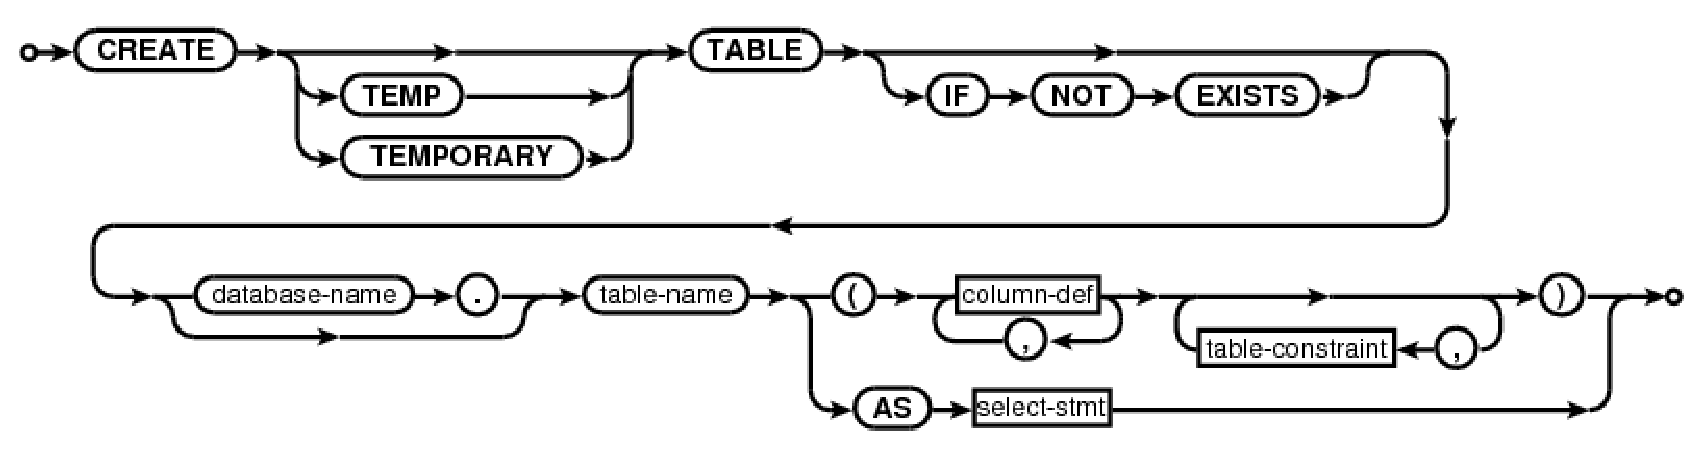
\includegraphics[scale=0.35]{create-table-stmt.eps}

\scriptsize column-def: \\
\vspace{4pt} 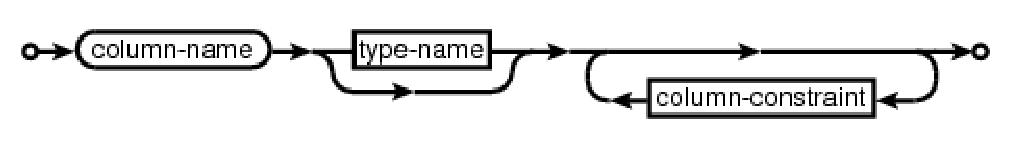
\includegraphics[scale=0.4]{column-def.eps}

%\scriptsize column-constraint: PRIMARY KEY, FOREIGN KEY, UNIQUE, \\

{\vspace{6pt} \tiny Ref: www.sqlite.org/lang\_createtable.html} 


\end{frame}
%%%%%%%%%%%%%%%%%%%%%%%%%%%%%%%%%%%
\begin{frame}{Example 1: Building \& Populating}

\begin{columns}
\column{0.45\textwidth} \scriptsize

{\bf Exemplifies:}
\begin{itemize} \setlength\itemindent{-5pt}%\itemsep-1pt
	\item Python
	\begin{itemize} \setlength\itemindent{-20pt} \scriptsize
		\item[$\bullet$] $sqlite3.connect()$
		\item[$\bullet$] $Connection.execute()$
		\item[$\bullet$] $Connection.commit()$
	\end{itemize}
	\item SQL
	\begin{itemize}\setlength\itemindent{-20pt} \scriptsize
		\item[$\bullet$] \textit{CREATE TABLE}
		\item[$\bullet$] \textit{INSERT INTO}
	\end{itemize}
\end{itemize}

\vspace{12pt}$connect()$ will create the file if it doesn't exist. If we need to change this behavior we can use python's $os.path.exist()$.

%\vspace{8pt} All fields except `$time$' are interpreted as SQLite TEXT datatype. \\
%{\tiny Ref: www.sqlite.org/datatype3.html} \\

\column{0.5\textwidth}
\lstinputlisting{../example1.py}
\end{columns}
\end{frame}
%%%%%%%%%%%%%%%%%%%%%%%%%%%%%%%%%%%
\begin{frame}{And query it!}

\textit{``Well how many Gold's did that Michael Phelps get?''}

\vspace{12pt}\hspace{4cm} Their's a query for that.

\vspace{12pt}
\large {\bf Outline:}
\begin{itemize}
\item SQL Select Query
\item Example 2: Select Queries
\end{itemize}

\end{frame}
%%%%%%%%%%%%%%%%%%%%%%%%%%%%%%%%%%%
\begin{frame}{SQL Select Query} \footnotesize 

\begin{columns}
\column{0.35\textwidth} \footnotesize

\vspace{8pt}The `SELECT' statement returns a result set from one or more tables. \\

\vspace{8pt}SQL is not case sensitive. \\

\vspace{8pt}Most programmers use capitals to denote SQL keywords but this is by practice only. \\

\vspace{8pt} 

\column{0.6\textwidth}

{\bf SELECT} \\
\vspace{4pt} 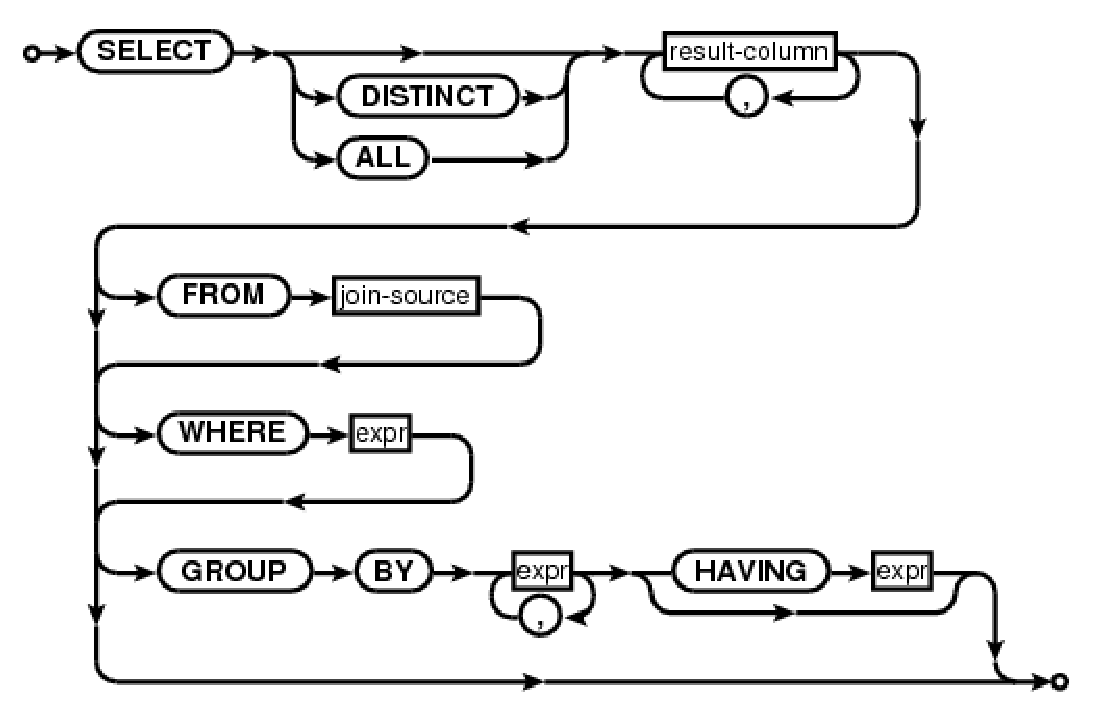
\includegraphics[scale=0.35]{select-core.eps}

{\vspace{6pt} \tiny Ref: www.sqlite.org/lang\_select.html} 

\end{columns}

\end{frame}

%%%%%%%%%%%%%%%%%%%%%%%%%%%%%%%%%%%
\begin{frame}{Example 2: Select Queries}

\begin{columns}
\column{0.45\textwidth} \scriptsize

{\bf Exemplifies:}
\begin{itemize} \setlength\itemindent{-5pt}%\itemsep-1pt
	\item Python
	\begin{itemize} \setlength\itemindent{-20pt} \scriptsize
		\item[$\bullet$] $Cursor.fetchone()$
		\item[$\bullet$] $Connection.text\_factory$
	\end{itemize}
	\item SQL
	\begin{itemize} \setlength\itemindent{-20pt} \scriptsize
		\item[$\bullet$] \textit{SELECT}
		\item[$\bullet$] \textit{WHERE}
	\end{itemize}
\end{itemize}

\vspace{12pt} The `$Connection.text\_factory$' property changes what type of object is returned from a SQLite TEXT datatype.

\column{0.5\textwidth}
\lstinputlisting{../example2.py}

\end{columns}

\end{frame}
%%%%%%%%%%%%%%%%%%%%%%%%%%%%%%%%%%%
\begin{frame}{And schema changes?}

\textit{``What if we want to change the schema?''}

\vspace{3pt}\hspace{.5cm} ``What if we want to alter a column in our table?''

\vspace{12pt}\hspace{2.5cm} Let's make the medal field case-insensitive.

\vspace{12pt}
\large {\bf Outline:}
\begin{itemize}
\item SQL Alter Table
\item SQL Alter Column
\item Example 3: Table Updates
\end{itemize}

\end{frame}
%%%%%%%%%%%%%%%%%%%%%%%%%%%%%%%%%%%
\begin{frame}{SQL Alter Table} \footnotesize 

\begin{columns}
\column{0.85\textwidth}

\vspace{6pt} SQLite supports a limited `ALTER TABLE' statement for:
\begin{itemize} \setlength\itemindent{-5pt}\itemsep-1pt
  \item Renaming tables
  \item Adding columns
\end{itemize}

\vspace{12pt} {\bf ALTER TABLE} \\
\vspace{4pt} 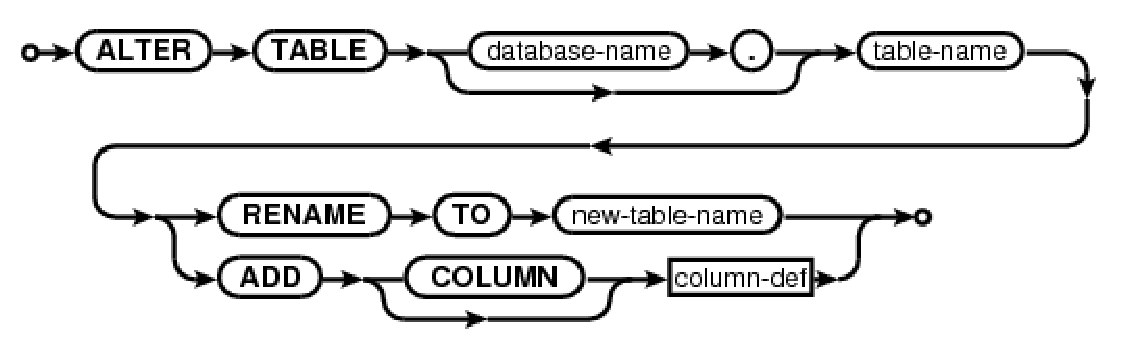
\includegraphics[scale=0.35]{alter-table-stmt.eps}

{\vspace{6pt} \tiny Ref: www.sqlite.org/lang\_altertable.html} 
\end{columns}

\end{frame}
%%%%%%%%%%%%%%%%%%%%%%%%%%%%%%%%%%%
\begin{frame}{SQL Alter Column} \footnotesize 

\vspace{8pt} SQLite supports no `ALTER COLUMN' statement.

\vspace{12pt} To do the behavior of an `ALTER COLUMN' we can:
\begin{enumerate} %\setlength\itemindent{-5pt}\itemsep-1pt
  \item Rename the table to a temporary name
  \item Create a new table with the corrected field
  \item Insert data from the old table into the new table
  \item Drop the old table
\end{enumerate}

\vspace{12pt} An alternative method exists via use of 'PRAGMA' statement but is unsafe and may corrupt the database.

\end{frame}
%%%%%%%%%%%%%%%%%%%%%%%%%%%%%%%%%%%
\begin{frame}{Example 3: Table Updates}

\begin{columns}
\column{0.43\textwidth} \scriptsize 
{\bf Exemplifies:}
\begin{itemize} \setlength\itemindent{-5pt}%\itemsep-1pt
	\item Python
	\begin{itemize} \setlength\itemindent{-20pt} \scriptsize
		\item[$\bullet$] $Connection.executescript()$
	\end{itemize}
	\item SQL
	\begin{itemize} \setlength\itemindent{-20pt} \scriptsize
		\item[$\bullet$] \textit{ALTER TABLE}
		\item[$\bullet$] \textit{DROP TABLE}
	\end{itemize} 
\end{itemize}

\vspace{12pt} We check that the medal field is now case-insensitive \textit{via} a query counting bronze and silver medals

\column{0.5\textwidth}
\lstinputlisting{../example3.py}

\end{columns}

\end{frame}
%%%%%%%%%%%%%%%%%%%%%%%%%%%%%%%%%%%
\begin{frame}{Helper objects?}

\vspace{2pt}\hspace{.5cm} ``Are there helper objects for mapping column names and datatypes to results?''

\vspace{12pt}\hspace{6.5cm} \Large{Yes.}

\vspace{12pt}
\large {\bf Outline:}
\begin{itemize}
\item Example 4: $sqlite3.Row$
\end{itemize}

\end{frame}
%%%%%%%%%%%%%%%%%%%%%%%%%%%%%%%%%%%
\begin{frame}{Example 4: $sqlite3.Row$}

\begin{columns}
\column{0.45\textwidth} \scriptsize

{\bf Exemplifies:}
\begin{itemize} \setlength\itemindent{-5pt}%\itemsep-1pt
	\item Python
	\begin{itemize} \setlength\itemindent{-20pt} \scriptsize
		\item[$\bullet$] $Connection.row\_factory$
		\item[$\bullet$] $sqlite3.Row$
	\end{itemize}
\end{itemize} 

\vspace{12pt} $\bf sqlite3.Row$
\begin{itemize} \setlength\itemindent{-5pt}%\itemsep-1pt
	\item Allows access \textit{via} column name and index
	\item The $keys()$ method returns a tuple of column names
	\item Using slice notation generates ``Not implemented yet'' exception
\end{itemize} 

%Results returned as $sqlite3.Row$ object can be accessed like a python dictionary. In addition, the values are converted to the appropriate python data types.

\column{0.5\textwidth}
\lstinputlisting{../example4.py}

\end{columns}
\end{frame}
%%%%%%%%%%%%%%%%%%%%%%%%%%%%%%%%%%%
\begin{frame}{We can rebuild it}

\textit{``What if we want to change the schema?''}

\vspace{3pt}\hspace{5cm} ... and we are willing to be \textit{risky}

\vspace{12pt} PRAGMA statements allow us to edit database features and data access control.

%\vspace{8pt} To demonstrate the usage of PRAGMA we are going to revist the alter column example earlier.

\vspace{12pt}
\large {\bf Outline:}
\begin{itemize}
\item Example 5: SQLite Master Table
\item Example 6: Edit Schema
\end{itemize}

\end{frame}
%%%%%%%%%%%%%%%%%%%%%%%%%%%%%%%%%%%
\begin{frame}{Example 5: SQLite Master Table}

\begin{columns}
\column{0.45\textwidth} \scriptsize 

{\bf Exemplifies:}
\begin{itemize} \setlength\itemindent{-5pt}%\itemsep-1t
	\item Python
	\begin{itemize} \setlength\itemindent{-20pt} \scriptsize
		\item[$\bullet$] $Connection.cursor()$
		\item[$\bullet$] $Cursor.execute()$
		\item[$\bullet$] $Cursor.description$
	\end{itemize}
\end{itemize}

\vspace{12pt} The `sqlite\_master' table stores the SQLite database's schema.

\vspace{12pt} {\bf `sqlite\_master' fields:}
\begin{itemize} \setlength\itemindent{-5pt}%\itemsep-1t
\item Type
\item Name
\item Tbl\_Name
\item Rootpage
\item SQL
\end{itemize}

\column{0.5\textwidth}
\lstinputlisting{../example5.py}

\end{columns}

\end{frame}
%%%%%%%%%%%%%%%%%%%%%%%%%%%%%%%%%%%
\begin{frame}{Example 6: Edit Schema}

\begin{columns}
\column{0.45\textwidth} \scriptsize 

{\bf Exemplifies:}
\begin{itemize} \setlength\itemindent{-5pt}%\itemsep-1pt
	\item SQL
	\begin{itemize} \setlength\itemindent{-20pt} \scriptsize
		\item[$\bullet$] \textit{PRAGMA}
		\item[$\bullet$] \textit{UPDATE}
	\end{itemize}
\end{itemize}

\vspace{12pt} ``Warning: misuse of this pragma can \textit{easily} result in a corrupt database file.''

\vspace{12pt} This potential exists because changes are made directly to the schema without any validation.

\column{0.5\textwidth}
\lstinputlisting{../example6.py}

\end{columns}

\end{frame}

%%%%%%%%%%%%%%%%%%%%%%%%%%%%%%%%%%%
\begin{frame}{Game changing data}

\vspace{.5cm} Since Michael Phelps is retiring, we've decided to add Ryan Lochte for tracking him in future olympic seasons.

\vspace{12pt}
\large {\bf Outline:}
\begin{itemize}
\item Lochte's Excel Data
\item Example 7: New Architecture
\item Example 8: New Data
\end{itemize}

\end{frame}
%%%%%%%%%%%%%%%%%%%%%%%%%%%%%%%%%%%
\begin{frame}{Lochte's Excel Data}
\includegraphics[scale=0.5]{lochte_table.pdf}
\end{frame}
%%%%%%%%%%%%%%%%%%%%%%%%%%%%%%%%%%%
\begin{frame}{Example 7: New Architecture }

\begin{columns}
\column{0.85\textwidth}
\lstinputlisting{../example7.py}

\end{columns}

\end{frame}
%%%%%%%%%%%%%%%%%%%%%%%%%%%%%%%%%%%
\begin{frame}{Example 8: New Data }

\begin{columns}
\column{0.85\textwidth}
\lstinputlisting{../example8.py}

\end{columns}

\end{frame}
%%%%%%%%%%%%%%%%%%%%%%%%%%%%%%%%%%%
\begin{frame}{As complexity grows}

\vspace{8pt}The major gains to relational databases are found when data is seperated into related tables.

\vspace{12pt}The process of optimizing databases by minimizing redudancy and dependency is known as \textit{database normalizaton}.

\vspace{12pt}
\large {\bf Outline:}
\begin{itemize}
\item Example 9: Normalization
\item Example 10: Making reports
\end{itemize}

\end{frame}
%%%%%%%%%%%%%%%%%%%%%%%%%%%%%%%%%%%
\begin{frame}{Example 9: Normalization }

\begin{columns}
\column{1.0\textwidth}
\lstinputlisting{../example9.py}

\end{columns}

\end{frame}
%%%%%%%%%%%%%%%%%%%%%%%%%%%%%%%%%%%
%%%%%%%%%%%%%%%%%%%%%%%%%%%%%%%%%%%
\begin{frame}{Example 10: Making Reports }

\begin{columns}
\column{1.0\textwidth}
\lstinputlisting{../example10.py}

\end{columns}

\end{frame}
%%%%%%%%%%%%%%%%%%%%%%%%%%%%%%%%%%%
\begin{frame}{Code packing}

\vspace{2pt}\hspace{.5cm} ``What if we want to  pack our code inside an sqlite database?''

\vspace{12pt}\hspace{6.5cm} \Large{Yes.}

\vspace{12pt}
\large {\bf Outline:}
\begin{itemize}
\item Example 11: BLOBs
\end{itemize}

\end{frame}
%%%%%%%%%%%%%%%%%%%%%%%%%%%%%%%%%%%
\begin{frame}{Example 11: BLOBs }

\begin{columns}
\column{1.0\textwidth}
\lstinputlisting{../example11.py}

\end{columns}

\end{frame}
%%%%%%%%%%%%%%%%%%%%%%%%%%%%%%%%%%%
\begin{frame}{Mapping \& Diagraming} \scriptsize

\normal As databases get more complex or multiple database dialets become involved, the need for more tools arises.

\vspace{16pt} \begin{columns}
\column{0.45\textwidth}
\normal {\bf Object-relational mapping (ORM) } \\
\begin{itemize} \setlength\itemindent{-5pt}%\itemsep-1pt
	\item Maps incompatible type systems
	\item Provides object-oriented access
	\item Often supports multiple dialects
\end{itemize}

\centering
\vspace{6pt} \normal {\bf Ex. }
SQLAlchemy \\
\vspace{2pt} www.sqlalchemy.org \\

\column{0.55\textwidth}
\normal {\bf Entity-relationship diagrams (ERD) } \\
\begin{itemize} \setlength\itemindent{-5pt}%\itemsep-1pt
	\item Show relationships within a database
	\item Contains entities, relationships, attributes
	\item May show cardinality of relationships
\end{itemize}

\centering
\vspace{6pt} \normal {\bf Ex. }
Open System Architect \\
\vspace{2pt} www.codebydesign.com \\

\end{columns}

\end{frame}
%%%%%%%%%%%%%%%%%%%%%%%%%%%%%%%%%%%

\begin{comment}
\begin{frame}{A sample slide}

A displayed formula:

\[
  \int_{-\infty}^\infty e^{-x^2} \, dx = \sqrt{\pi}
\]

An itemized list:

\begin{itemize}
  \item itemized item 1
  \item itemized item 2
  \item itemized item 3
\end{itemize}

\begin{theorem}
  In a right triangle, the square of hypotenuse equals
  the sum of squares of two other sides.
\end{theorem}

\end{frame}
\end{comment}


\end{document}